% REMEMBER: You must not plagiarise anything in your report. Be extremely careful.

\documentclass{l4proj}

    
%
% put any additional packages here
\usepackage{siunitx}
%

\begin{document}

%==============================================================================
%% METADATA
\title{Using Deep Learning to predict overall survival times for breast cancer from H\&E stained whole slide biopsy images}
\author{Anirbit Ghosh}
\date{September 14, 2022}

\maketitle

%==============================================================================
%% ABSTRACT
\begin{abstract}
    Current pathological practice to diagnose malignancy involves the manual identification and annotation of the extent of cancerous tumour cells in a biopsy slide image by a trained pathologist. This process is highly resource intensive and is subject to the interpretation variability between different readers leading to inconsistent outcomes. Therefore a Deep Learning based automated cancer detection system which can accurately and robustly identify the extent of malignancy from the digital whole slide image would be a highly desirable and potentially industry changing advancement. The subsequent step after the initial cancer diagnosis requires vast amounts of the patient's clinical data to be collected and processed in order to deliver a survival time prediction. The clinical data required to produce a survival time model for a patient ranges from general health and quality of life measures to specific characteristics of the malignant areas which must be extracted manually by pathologists. Given the sensitive nature of a cancer diagnosis in the first place it is often of essence to avoid putting patients through extensive diagnostic tests and data collection only to deliver potentially worse news with the survival time prognosis. Biopsy slide images hold a plethora of cellular level and structural information which can very effectively help understand the exact nature of malignancy. However, manually analyzing whole slide images to extract useful features is extremely expensive in terms of time and storage due to the sheer size of these images. Thus, augmenting the Deep Learning based cancer detection system to automatically extract useful features from the digital biopsy images can aid in characterizing cancer severity and giving a survival time estimate without the need of vast amounts of clinical data. The biggest problem in creating this system is the lack of annotated patient biopsy data that is publicly available, which makes effectively training a network to automatically detect malignant tissue extremely challenging. In this project, I proposed training a deep neural network on the Camelyon 16 data, which is a collection of 170 weakly annotated lymph node whole slide images from breast cancer patients. Breast cancer frequently metastasizes to axillary lymph nodes which makes them a good prognostic factor of breast cancer severity. The data contained 70 metastatic and 100 non-metastatic whole slides giving a good balance of positive and negative samples to train the network to accurately segment cancerous cells from a given tissue image. This process was a very unusual approach as there is no existing literature verifying the validity of using a network trained on breast metastasis found in lymph node tissue to detect malignancy in breast tissue. The different tissue composition posed a significant risk of complete network failure. However, the results showed surprisingly accurate and reasonable outcomes indicating that metastasis characterization transfers across multiple tissue types. The survival model was then generated using whole slide images of patients available on TCGA by processing their biopsies through the trained network and extracting features to characterize malignancy levels. The generated features were used as a heuristic in conjunction with each patient's predicted survival times (from associated clinical data) to generate a Cox Proportional-hazard model which is a regression model that can generates a survival time for a given heuristic level.  
    
\end{abstract}

%==============================================================================

% EDUCATION REUSE CONSENT FORM
% If you consent to your project being shown to future students for educational purposes
% then insert your name and the date below to  sign the education use form that appears in the front of the document. 
% You must explicitly give consent if you wish to do so.
% If you sign, your project may be included in the Hall of Fame if it scores particularly highly.
%
% Please note that you are under no obligation to sign 
% this declaration, but doing so would help future students.
%
\def\consentname {Anirbit Ghosh} % your full name
\def\consentdate {20 March 2022} % the date you agree
%
\educationalconsent


%==============================================================================
\tableofcontents

%==============================================================================
%% Notes on formatting
%==============================================================================
% The first page, abstract and table of contents are numbered using Roman numerals and are not
% included in the page count. 
%
% From now on pages are numbered
% using Arabic numerals. Therefore, immediately after the first call to \chapter we need the call
% \pagenumbering{arabic} and this should be called once only in the document. 
%
% The first Chapter should then be on page 1. You are allowed 40 pages for a 40 credit project and 20 pages for a 
% 20 credit report. This includes everything numbered in Arabic numerals (excluding front matter) up
% to but excluding the appendices and bibliography.
%
% You must not alter text size (it is currently 10pt) or alter margins or spacing.
%
%
%==================================================================================================================================
%
% IMPORTANT
% The chapter headings here are **suggestions**. You don't have to follow this model if
% it doesn't fit your project. Every project should have an introduction and conclusion,
% however. 
%
%==================================================================================================================================
\chapter{Introduction}

% reset page numbering. Don't remove this!
\pagenumbering{arabic} 

\section{Motivation}
With a global estimate of 18 million cases [1] of cancer diagnosed each year, as of 2020, female breast cancer has become the most common contributor making up over 12.5\% [2] of all cases of which 684,996 [3] cases were fatal making it the fifth leading cause of death. However, with an average 75\% 10-year survival rate across all stages of breast cancer [4], it shows the best prospects for generally being the most curable form provided an early diagnosis followed by appropriate and timely treatment. This constitutes the rationale for focusing this dissertation on improving the efficiency of breast cancer diagnosis and prognosis prediction. 

A biopsy is the only definitive way of diagnosing breast cancer. Traditionally a trained pathologist would be required to manually inspect a biopsied tissue sample and identify potential areas  abnormal, malignant cell growth. Subsequently an oncologist would use this pathology report to determine the patient's prognosis in terms of likelihood of recovery and survival chance which guides the course of treatment. Classical prognosis prediction  relies on population-level estimates by comparing a patient's case to previously documented similar cases based on cancer site, tumour grade, cancer stage and certain cellular markers. As every patient's cancer manifests uniquely, this technique is further supplemented by collecting the individual patient's clinical and quality of life information combined with several test results of multiple bio-markers. This complete diagnostic workflow is not only time consuming but also highly subjective and non-reproducible due to vast amount of data required to characterize each patient's condition and the manual effort required to produce and interpret that data.

If the delay between tissue collection, diagnosis and subsequent prognosis prediction could be minimized, it would allow patients to receive the appropriate treatment much quicker which can increase the likelihood of recovery in particularly time sensitive cases. Furthermore, reducing human involvement in the diagnostic procedure can eliminate interpretation variability making diagnoses more consistent and robust. As severe as it maybe, this will allow patients to be more confident in their first prognosis and eliminate the need to get a second opinion which in most cases serves as an unnecessary delay to starting the much needed treatment which could help increase their survival prospects. 


\section{General problem and our hypothesis}
The biopsied sample of breast tissue used in the diagnostic process is an exact characterization of the patient's individual condition. The structural and cellular level information obtained from biopsies is very valuable in understanding the extent and severity of cancer. A digital representation of the biopsied tissue can be obtained in the form a whole slide image (WSI), which is a high resolution, multi-level replication of the stained tissue as observed under a microscope at varying zoom levels. These digital slide images can be used in an automated cancer diagnostic system by treating the detection of malignant cells in the image as a classification problem. 

The general problem we are attempting to solve is to utilize digital whole slide images of biopsied tissue to automate the diagnosis of breast cancer without requiring manual annotation of tissue slides by pathologists. Furthermore, we are attempting to estimate the patient's prognosis in terms of an overall survival time by utilizing information extracted from the whole slide image, thereby eliminating the dependence on extensive clinical data collection and analysis. 

This paper proposes a supervised learning model which will be trained with patches of breast cancer whole slide images to learn how to perform slide level classification of malignant and benign tissue. Subsequently, we develop and extract some image-based features from the segmented whole slide images to predict an estimate for the survival time of the given patient. 



\section{Aim}
This project aims to investigate the viability of deep-learning based automated breast cancer diagnosis and corresponding survival time  prediction only using digital slide images of the affected tissue. We are trying to minimize or potentially eliminate the requirement of manual human intervention and vast amounts of clinical data in the diagnostic process. The project will achieve this by performing the following tasks:

\begin{itemize}
    \item
    elaborate the idea of automated cancer detection from whole slide images and describe the problem of inferring an estimated disease prognosis from a single slide image. 
    \item 
    prepare a training dataset with fixed size patches of whole slide images of breast tissue samples along with patch-level annotations for malignancy or benignity. The dataset must be standardized to eliminate any impact of human variability involved in the preparation of tissue slides collected from various sources.
    \item
    implement and train a supervised learning based deep convolutional neural network that can learn to distinguish between malignant and benign breast tissue. It will accept patches of a whole slide image and output a fully segmented whole slide image showing areas of malignancy.
    \item
    develop and extract a feature metric from the segmented whole slide image to quantify and characterize the nature of breast cancer in a given tissue slide. Using this metric, generate a statistical model to predict a proportional survival time for any given case. 
    \item
    evaluate the performance of the cancer detection network against clinically annotated ground truth samples. Measure accuracy of survival time prediction against available clinical data and infer validity of exclusively using whole slide images in delivering disease prognosis. 
\end{itemize}

%==================================================================================================================================
\chapter{Background}

\section{Whole Slide Images}
\subsection{Slide preparation}
Biopsied tissue blocks are sliced into thin sections and mounted on glass slides. These tissue slides are generally stained with a Hematoxylin and Eosin dye which has been proven (\textit{\cite{Bancroft2013}}) to exhibit the ability to highlight a wide range of diagnostic cellular artifacts which are otherwise not visible under digital microscopy.  In breast tissue, the Hematoxylin component stains the nuclei of cells in a blue colour as it binds to acidic structures, particularly RNA and DNA (\textit{\cite{chan2014wonderful}}). Eosin on the contrary stains any connective tissue and cellular cytoplasm in shades of red (\textit{\cite{Bancroft2013}}), which in breast tissue samples makes up the majority of the surface due to the presence of muscles, fatty tissue and collagen. Collagen is the dominant component in tissue surrounding breast ducts which is the most common area of origin for breast cancer making this staining even more effective in distinguishing between normal and abnormal cellular growth. Therefore, H\&E staining has become the histopathology standard when diagnosing breast cancer from biopsied tissue.

\begin{figure}[h]
\centering
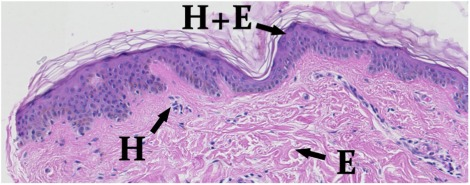
\includegraphics[scale=1.2]{images/HE-stain-example.jpg}
\caption{section of skin showing Hematoxylin(H) \& Eosin(E) stain interactions}
\label{fig:HE-fig}
\end{figure}

\subsection{Slide digitization}
Physical tissue slides are digitized using whole slide image scanners which contain an illumination system, an optical microscope and a focusing apparatus (\textit{\cite{ghaznavi2013digital}}). Scanners most commonly use Brightfield illumination (\textit{\cite{kino1996confocal}}) in which the entire tissue sample is uniformly illuminated. This works in conjunction with the H\&E staining to display the tissue as a dark coloured image on a white background making it easier to distinguish cellular structure. 

The final output of the slide scanner is a virtual rendering of the entire tissue slide, that can be viewed at resolutions of upto 0.25 \si{\micro\meter} corresponding to a 40x objective power of the scanning microscope. In order to replicate a slide under a microscope, WSIs exhibit a pyramid structure consisting of images at multiple resolutions. The base level stores the image in diagnostic resolution of a 40x objective, often containing 100,000 x 100,000 pixels (\textit{\cite{wang2012managing}}). As displayed in figure(\ref{fig:pyramid-fig}) The resolution is down sampled by a fixed factor at each subsequent level. The Cancer Genome Atlas program's repository contains WSIs with 4 resolution levels down-sampled with factors of 1.0, 4.0, 16.0 and 64.0. This feature of WSIs makes these images extremely bulky with average sizes around 1GB per image. 

\begin{figure}[h]
\centering
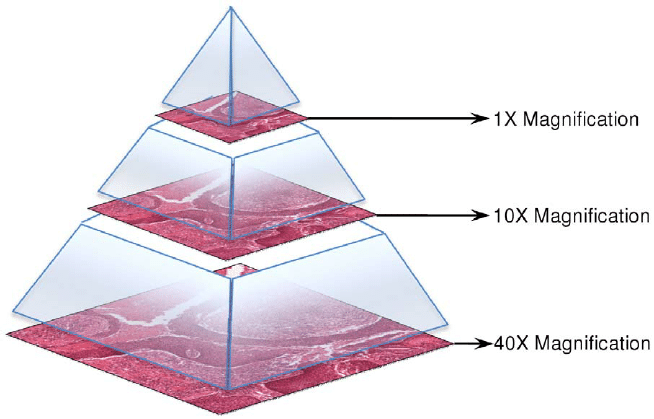
\includegraphics[scale=0.5]{images/digital-slide-stored-in-a-pyramid-structure.png}
\caption{Illustration of pyramid structure observed in whole slide images. Highest resolution at 40x magnification followed by 2 downsampled levels at 4.0 (10x) and 40.0 (1x)}
\label{fig:pyramid-fig}
\end{figure}

Viewing or analyzing an entire WSI is infeasible as the whole image simply cannot fit into a standard computer's memory. It was demonstrated by \cite{wang2012managing} that sectioning the WSI into several smaller, fixed size tiles at its diagnostic resolution and performing image analysis tasks on each tile allows for more efficient processing compared to using the entire slide image at once. As shown by \cite{aeffner2019introduction}, confining analysis efforts to smaller regions of interest (ROIs) rather than the entire WSI is often necessary to devise any accurate or computationally viable image analysis algorithms. The tile based results can be aggregated in order to generate masks that highlight all ROIs on lower resolution thumbnails of the original WSI in order to display the results of our image analysis tasks. 

\subsection{Slide normalization}

%==================================================================================================================================
\chapter{Analysis/Requirements}
What is the problem that you want to solve, and how did you arrive at it?
\section{Guidance}
Make it clear how you derived the constrained form of your problem via a clear and logical process. 

%==================================================================================================================================
\chapter{Design}
How is this problem to be approached, without reference to specific implementation details? 
\section{Guidance}
Design should cover the abstract design in such a way that someone else might be able to do what you did, but with a different language or library or tool.

%==================================================================================================================================
\chapter{Implementation}
What did you do to implement this idea, and what technical achievements did you make?
\section{Guidance}
You can't talk about everything. Cover the high level first, then cover important, relevant or impressive details.



\section{General points}

These points apply to the whole dissertation, not just this chapter.



\subsection{Figures}
\emph{Always} refer to figures included, like Figure \ref{fig:relu}, in the body of the text. Include full, explanatory captions and make sure the figures look good on the page.
You may include multiple figures in one float, as in Figure \ref{fig:synthetic}, using \texttt{subcaption}, which is enabled in the template.



% Figures are important. Use them well.
\begin{figure}
    \centering
    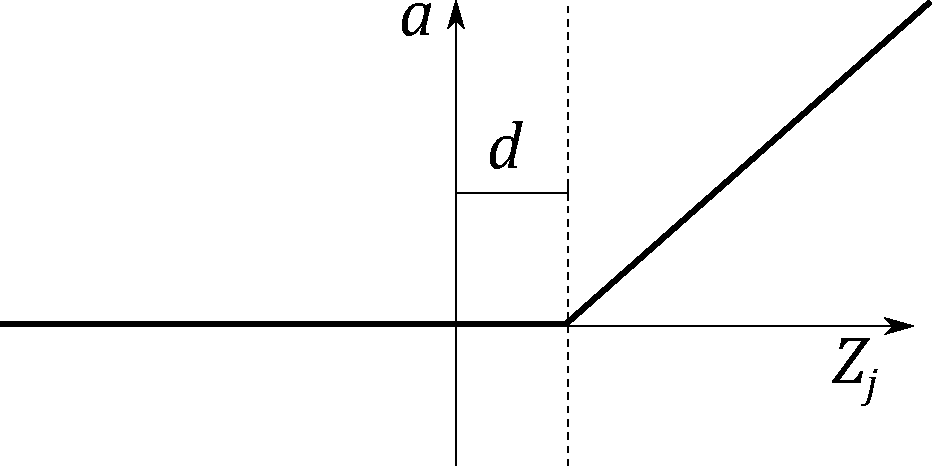
\includegraphics[width=0.5\linewidth]{images/relu.pdf}    

    \caption{In figure captions, explain what the reader is looking at: ``A schematic of the rectifying linear unit, where $a$ is the output amplitude,
    $d$ is a configurable dead-zone, and $Z_j$ is the input signal'', as well as why the reader is looking at this: 
    ``It is notable that there is no activation \emph{at all} below 0, which explains our initial results.'' 
    \textbf{Use vector image formats (.pdf) where possible}. Size figures appropriately, and do not make them over-large or too small to read.
    }

    % use the notation fig:name to cross reference a figure
    \label{fig:relu} 
\end{figure}


\begin{figure}
    \centering
    \begin{subfigure}[b]{0.45\textwidth}
        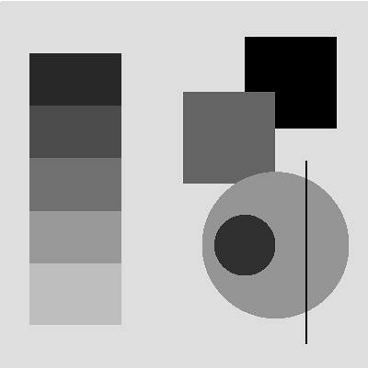
\includegraphics[width=\textwidth]{images/synthetic.png}
        \caption{Synthetic image, black on white.}
        \label{fig:syn1}
    \end{subfigure}
    ~ %add desired spacing between images, e. g. ~, \quad, \qquad, \hfill etc. 
      %(or a blank line to force the subfigure onto a new line)
    \begin{subfigure}[b]{0.45\textwidth}
        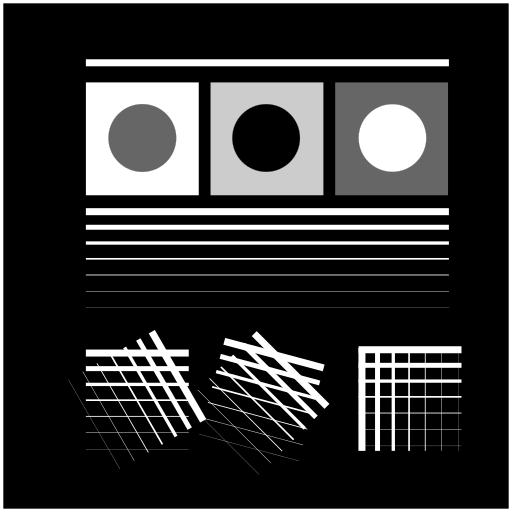
\includegraphics[width=\textwidth]{images/synthetic_2.png}
        \caption{Synthetic image, white on black.}
        \label{fig:syn2}
    \end{subfigure}
    ~ %add desired spacing between images, e. g. ~, \quad, \qquad, \hfill etc. 
    %(or a blank line to force the subfigure onto a new line)    
    \caption{Synthetic test images for edge detection algorithms. \subref{fig:syn1} shows various gray levels that require an adaptive algorithm. \subref{fig:syn2}
    shows more challenging edge detection tests that have crossing lines. Fusing these into full segments typically requires algorithms like the Hough transform.
    This is an example of using subfigures, with \texttt{subref}s in the caption.
    }\label{fig:synthetic}
\end{figure}

\clearpage

\subsection{Equations}

Equations should be typeset correctly and precisely. Make sure you get parenthesis sizing correct, and punctuate equations correctly 
(the comma is important and goes \textit{inside} the equation block). Explain any symbols used clearly if not defined earlier. 

For example, we might define:
\begin{equation}
    \hat{f}(\xi) = \frac{1}{2}\left[ \int_{-\infty}^{\infty} f(x) e^{2\pi i x \xi} \right],
\end{equation}    
where $\hat{f}(\xi)$ is the Fourier transform of the time domain signal $f(x)$.

\subsection{Algorithms}
Algorithms can be set using \texttt{algorithm2e}, as in Algorithm \ref{alg:metropolis}.

% NOTE: line ends are denoted by \; in algorithm2e
\begin{algorithm}
    \DontPrintSemicolon
    \KwData{$f_X(x)$, a probability density function returing the density at $x$.\; $\sigma$ a standard deviation specifying the spread of the proposal distribution.\;
    $x_0$, an initial starting condition.}
    \KwResult{$s=[x_1, x_2, \dots, x_n]$, $n$ samples approximately drawn from a distribution with PDF $f_X(x)$.}
    \Begin{
        $s \longleftarrow []$\;
        $p \longleftarrow f_X(x)$\;
        $i \longleftarrow 0$\;
        \While{$i < n$}
        {
            $x^\prime \longleftarrow \mathcal{N}(x, \sigma^2)$\;
            $p^\prime \longleftarrow f_X(x^\prime)$\;
            $a \longleftarrow \frac{p^\prime}{p}$\;
            $r \longleftarrow U(0,1)$\;
            \If{$r<a$}
            {
                $x \longleftarrow x^\prime$\;
                $p \longleftarrow f_X(x)$\;
                $i \longleftarrow i+1$\;
                append $x$ to $s$\;
            }
        }
    }
    
\caption{The Metropolis-Hastings MCMC algorithm for drawing samples from arbitrary probability distributions, 
specialised for normal proposal distributions $q(x^\prime|x) = \mathcal{N}(x, \sigma^2)$. The symmetry of the normal distribution means the acceptance rule takes the simplified form.}\label{alg:metropolis}
\end{algorithm}

\subsection{Tables}

If you need to include tables, like Table \ref{tab:operators}, use a tool like https://www.tablesgenerator.com/ to generate the table as it is
extremely tedious otherwise. 

\begin{table}[]
    \caption{The standard table of operators in Python, along with their functional equivalents from the \texttt{operator} package. Note that table
    captions go above the table, not below. Do not add additional rules/lines to tables. }\label{tab:operators}
    %\tt 
    \rowcolors{2}{}{gray!3}
    \begin{tabular}{@{}lll@{}}
    %\toprule
    \textbf{Operation}    & \textbf{Syntax}                & \textbf{Function}                            \\ %\midrule % optional rule for header
    Addition              & \texttt{a + b}                          & \texttt{add(a, b)}                                    \\
    Concatenation         & \texttt{seq1 + seq2}                    & \texttt{concat(seq1, seq2)}                           \\
    Containment Test      & \texttt{obj in seq}                     & \texttt{contains(seq, obj)}                           \\
    Division              & \texttt{a / b}                          & \texttt{div(a, b) }  \\
    Division              & \texttt{a / b}                          & \texttt{truediv(a, b) } \\
    Division              & \texttt{a // b}                         & \texttt{floordiv(a, b)}                               \\
    Bitwise And           & \texttt{a \& b}                         & \texttt{and\_(a, b)}                                  \\
    Bitwise Exclusive Or  & \texttt{a \textasciicircum b}           & \texttt{xor(a, b)}                                    \\
    Bitwise Inversion     & \texttt{$\sim$a}                        & \texttt{invert(a)}                                    \\
    Bitwise Or            & \texttt{a | b}                          & \texttt{or\_(a, b)}                                   \\
    Exponentiation        & \texttt{a ** b}                         & \texttt{pow(a, b)}                                    \\
    Identity              & \texttt{a is b}                         & \texttt{is\_(a, b)}                                   \\
    Identity              & \texttt{a is not b}                     & \texttt{is\_not(a, b)}                                \\
    Indexed Assignment    & \texttt{obj{[}k{]} = v}                 & \texttt{setitem(obj, k, v)}                           \\
    Indexed Deletion      & \texttt{del obj{[}k{]}}                 & \texttt{delitem(obj, k)}                              \\
    Indexing              & \texttt{obj{[}k{]}}                     & \texttt{getitem(obj, k)}                              \\
    Left Shift            & \texttt{a \textless{}\textless b}       & \texttt{lshift(a, b)}                                 \\
    Modulo                & \texttt{a \% b}                         & \texttt{mod(a, b)}                                    \\
    Multiplication        & \texttt{a * b}                          & \texttt{mul(a, b)}                                    \\
    Negation (Arithmetic) & \texttt{- a}                            & \texttt{neg(a)}                                       \\
    Negation (Logical)    & \texttt{not a}                          & \texttt{not\_(a)}                                     \\
    Positive              & \texttt{+ a}                            & \texttt{pos(a)}                                       \\
    Right Shift           & \texttt{a \textgreater{}\textgreater b} & \texttt{rshift(a, b)}                                 \\
    Sequence Repetition   & \texttt{seq * i}                        & \texttt{repeat(seq, i)}                               \\
    Slice Assignment      & \texttt{seq{[}i:j{]} = values}          & \texttt{setitem(seq, slice(i, j), values)}            \\
    Slice Deletion        & \texttt{del seq{[}i:j{]}}               & \texttt{delitem(seq, slice(i, j))}                    \\
    Slicing               & \texttt{seq{[}i:j{]}}                   & \texttt{getitem(seq, slice(i, j))}                    \\
    String Formatting     & \texttt{s \% obj}                       & \texttt{mod(s, obj)}                                  \\
    Subtraction           & \texttt{a - b}                          & \texttt{sub(a, b)}                                    \\
    Truth Test            & \texttt{obj}                            & \texttt{truth(obj)}                                   \\
    Ordering              & \texttt{a \textless b}                  & \texttt{lt(a, b)}                                     \\
    Ordering              & \texttt{a \textless{}= b}               & \texttt{le(a, b)}                                     \\
    % \bottomrule
    \end{tabular}
    \end{table}
\subsection{Code}

Avoid putting large blocks of code in the report (more than a page in one block, for example). Use syntax highlighting if possible, as in Listing \ref{lst:callahan}.

\begin{lstlisting}[language=python, float, caption={The algorithm for packing the $3\times 3$ outer-totalistic binary CA successor rule into a 
    $16\times 16\times 16\times 16$ 4 bit lookup table, running an equivalent, notionally 16-state $2\times 2$ CA.}, label=lst:callahan]
    def create_callahan_table(rule="b3s23"):
        """Generate the lookup table for the cells."""        
        s_table = np.zeros((16, 16, 16, 16), dtype=np.uint8)
        birth, survive = parse_rule(rule)

        # generate all 16 bit strings
        for iv in range(65536):
            bv = [(iv >> z) & 1 for z in range(16)]
            a, b, c, d, e, f, g, h, i, j, k, l, m, n, o, p = bv

            # compute next state of the inner 2x2
            nw = apply_rule(f, a, b, c, e, g, i, j, k)
            ne = apply_rule(g, b, c, d, f, h, j, k, l)
            sw = apply_rule(j, e, f, g, i, k, m, n, o)
            se = apply_rule(k, f, g, h, j, l, n, o, p)

            # compute the index of this 4x4
            nw_code = a | (b << 1) | (e << 2) | (f << 3)
            ne_code = c | (d << 1) | (g << 2) | (h << 3)
            sw_code = i | (j << 1) | (m << 2) | (n << 3)
            se_code = k | (l << 1) | (o << 2) | (p << 3)

            # compute the state for the 2x2
            next_code = nw | (ne << 1) | (sw << 2) | (se << 3)

            # get the 4x4 index, and write into the table
            s_table[nw_code, ne_code, sw_code, se_code] = next_code

        return s_table

\end{lstlisting}

%==================================================================================================================================
\chapter{Evaluation} 
How good is your solution? How well did you solve the general problem, and what evidence do you have to support that?

\section{Guidance}
\begin{itemize}
    \item
        Ask specific questions that address the general problem.
    \item
        Answer them with precise evidence (graphs, numbers, statistical
        analysis, qualitative analysis).
    \item
        Be fair and be scientific.
    \item
        The key thing is to show that you know how to evaluate your work, not
        that your work is the most amazing product ever.
\end{itemize}

\section{Evidence}
Make sure you present your evidence well. Use appropriate visualisations, reporting techniques and statistical analysis, as appropriate.

If you visualise, follow the basic rules, as illustrated in Figure \ref{fig:boxplot}:
\begin{itemize}
\item Label everything correctly (axis, title, units).
\item Caption thoroughly.
\item Reference in text.
\item \textbf{Include appropriate display of uncertainty (e.g. error bars, Box plot)}
\item Minimize clutter.
\end{itemize}

See the file \texttt{guide\_to\_visualising.pdf} for further information and guidance.

\begin{figure}
    \centering
    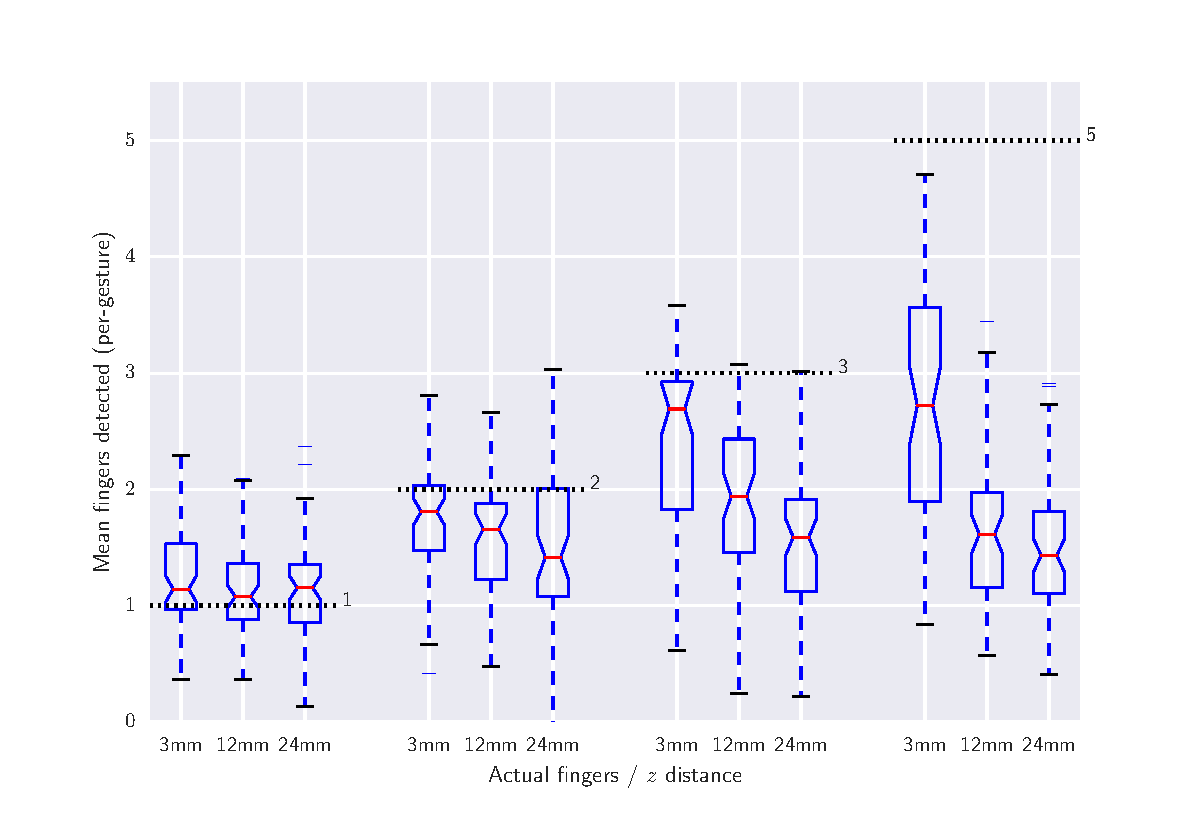
\includegraphics[width=1.0\linewidth]{images/boxplot_finger_distance.pdf}    

    \caption{Average number of fingers detected by the touch sensor at different heights above the surface, averaged over all gestures. Dashed lines indicate
    the true number of fingers present. The Box plots include bootstrapped uncertainty notches for the median. It is clear that the device is biased toward 
    undercounting fingers, particularly at higher $z$ distances.
    }

    % use the notation fig:name to cross reference a figure
    \label{fig:boxplot} 
\end{figure}


%==================================================================================================================================
\chapter{Conclusion}    
Summarise the whole project for a lazy reader who didn't read the rest (e.g. a prize-awarding committee).
\section{Guidance}
\begin{itemize}
    \item
        Summarise briefly and fairly.
    \item
        You should be addressing the general problem you introduced in the
        Introduction.        
    \item
        Include summary of concrete results (``the new compiler ran 2x
        faster'')
    \item
        Indicate what future work could be done, but remember: \textbf{you
        won't get credit for things you haven't done}.
\end{itemize}

%==================================================================================================================================
%
% 
%==================================================================================================================================
%  APPENDICES  

\begin{appendices}

\chapter{Appendices}

Typical inclusions in the appendices are:

\begin{itemize}
\item
  Copies of ethics approvals (required if obtained)
\item
  Copies of questionnaires etc. used to gather data from subjects.
\item
  Extensive tables or figures that are too bulky to fit in the main body of
  the report, particularly ones that are repetitive and summarised in the body.

\item Outline of the source code (e.g. directory structure), or other architecture documentation like class diagrams.

\item User manuals, and any guides to starting/running the software.

\end{itemize}

\textbf{Don't include your source code in the appendices}. It will be
submitted separately.

\end{appendices}

%==================================================================================================================================
%   BIBLIOGRAPHY   

% The bibliography style is abbrvnat
% The bibliography always appears last, after the appendices.

\bibliographystyle{abbrvnat}

\bibliography{l4proj}

\end{document}
